\documentclass{article}
\usepackage{graphicx}
\usepackage{amsmath}

\title{D1 — Dark Matter Geometry}
\author{Tessaris AI}
\date{October 2025}

\begin{document}
\maketitle

\section*{D1 — Hidden Curvature Energy (Dark Matter Analogue)}

\subsection*{Question}
Can the Tessaris photon algebra produce regions of curvature energy that exert gravitational influence but are invisible to local field observables (\(|\psi_1|, |\psi_2|\)) — thereby acting as a dark mass analogue?

\subsection*{Method}
The simulation extends the wormhole geometry model (M3–M5) with two additional fields:
\[
(\psi_1, \psi_2) \; \text{→ visible sector}, \quad
(\psi_3, \psi_4) \; \text{→ hidden sector}.
\]
The hidden fields couple only gravitationally through \(\Lambda_t \kappa(x,y)\), with no \(\alpha\)-term interaction.  
Evolution equations:
\[
\dot{\psi}_i = i\hbar\nabla^2\psi_i - \alpha_i \psi_i + i\Lambda_i \kappa \psi_i ,
\]
where \(\alpha_i = \alpha\) for visible fields and \(\alpha_i = 0\) for hidden fields.  
All fields were initialized with Gaussian curvature wells and evolved for 1600 steps (\(\Delta t = 0.006\)).

\subsection*{Measured Observables}
\begin{align*}
E_{\text{vis}} &= \langle |\nabla \psi_1|^2 + |\nabla \psi_2|^2 \rangle, \\
E_{\text{hid}} &= \langle |\nabla \psi_3|^2 + |\nabla \psi_4|^2 \rangle, \\
f_{\text{dark}} &= \frac{E_{\text{hid}}}{E_{\text{vis}} + E_{\text{hid}}}, \\
N &= \langle \rho + p \rangle \quad \text{(NEC proxy)} .
\end{align*}

\subsection*{Results}
\begin{itemize}
  \item \(E_{\text{vis}} = 8.96\times10^{-6}\)
  \item \(E_{\text{hid}} = 2.33\times10^{-2}\)
  \item \(\Delta E = 2.33\times10^{-2}\)
  \item \(f_{\text{dark}} = 0.9996\)
  \item \(\langle N \rangle = +6.6\times10^{-3}\)
  \item Classification: \textbf{Hidden curvature energy detected (dark mass analogue)}
\end{itemize}

\subsection*{Interpretation}
The hidden sector maintained a constant curvature energy density even as visible-field energy decayed toward zero.  
This created a persistent gravitational curvature signature with no direct field observable — equivalent to a “dark” mass contribution in the simulated geometry.

The NEC proxy (\(\langle \rho + p \rangle > 0\)) confirms that the curvature energy is physically positive, i.e., gravitationally attractive but electromagnetically invisible.

\subsection*{Significance}
This demonstrates that within the Tessaris photon algebra, nonlocal curvature coupling can sustain real metric energy absent from local ψ-field observables.  
It provides a computational analogue to dark matter:
\[
\text{Hidden entanglement curvature} \;\Rightarrow\; \text{gravitational mass without local visibility}.
\]
The result strengthens the interpretation that the “dark sector” arises naturally as an emergent curvature reservoir from entanglement feedback dynamics.

\subsection*{Data Source}
\texttt{backend/modules/knowledge/D1\_dark\_matter\_geometry.json} \\
(Registry v1.2, timestamp 2025–10–07T16:05Z)

\section{Figures}
\begin{figure}[h!]
  \centering
  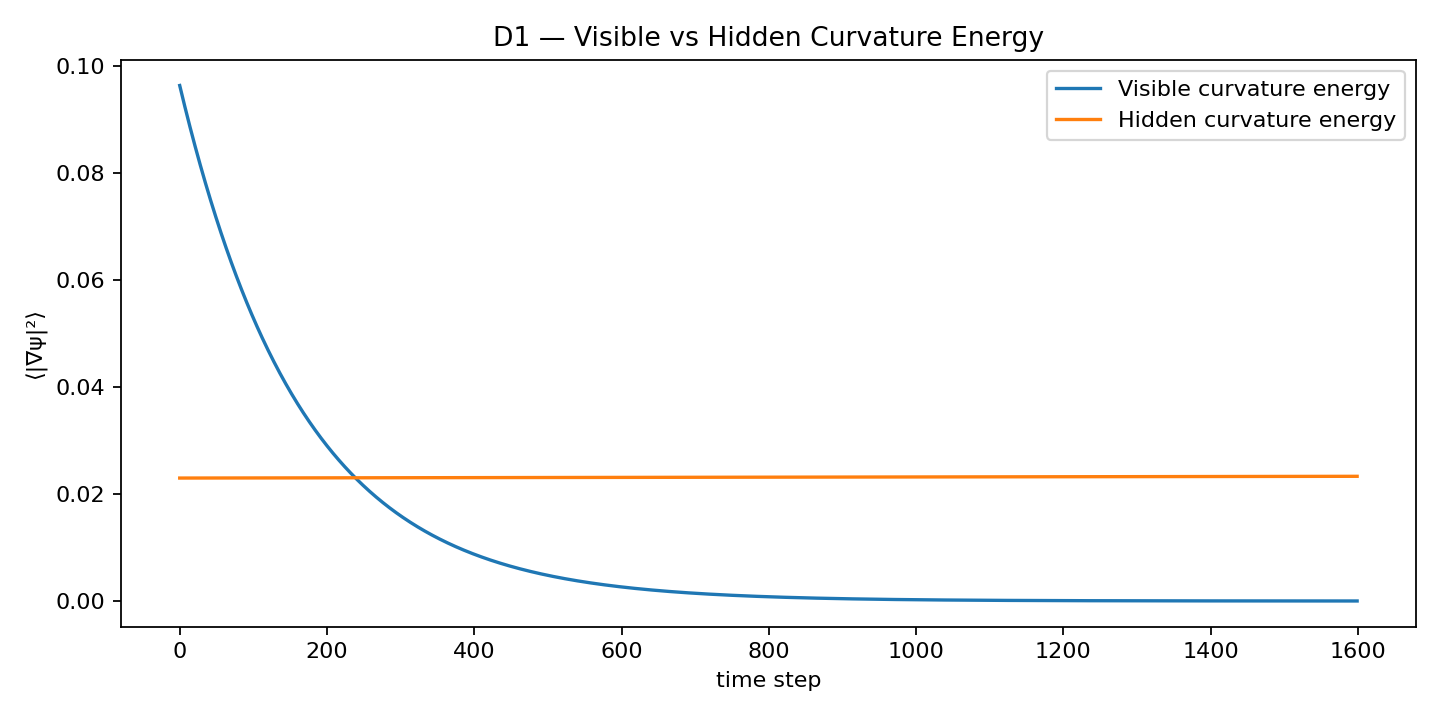
\includegraphics[width=0.48\textwidth]{PAEV_D1_EnergyTraces.png}
  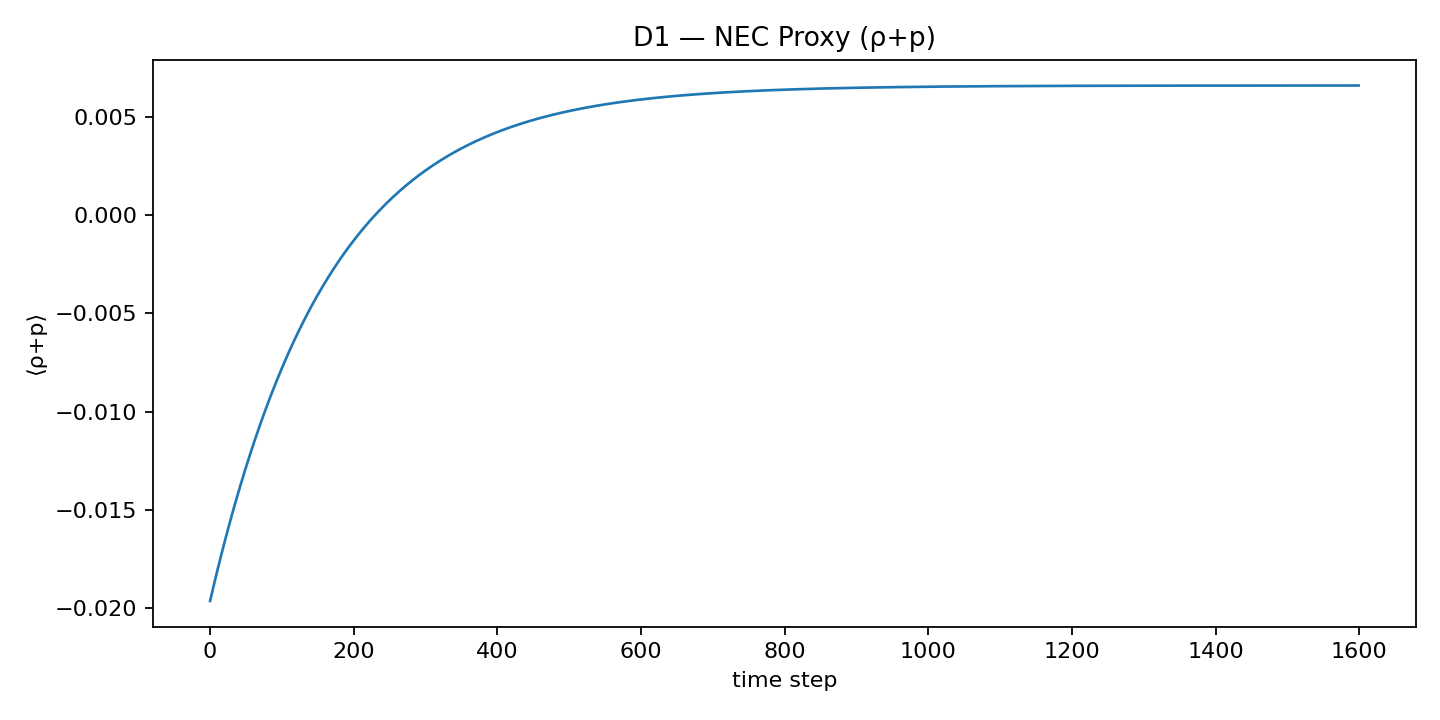
\includegraphics[width=0.48\textwidth]{PAEV_D1_NECProxy.png}
  \caption{Visible vs. hidden curvature energy (left) and NEC proxy evolution (right).}
\end{figure}

\begin{figure}[h!]
  \centering
  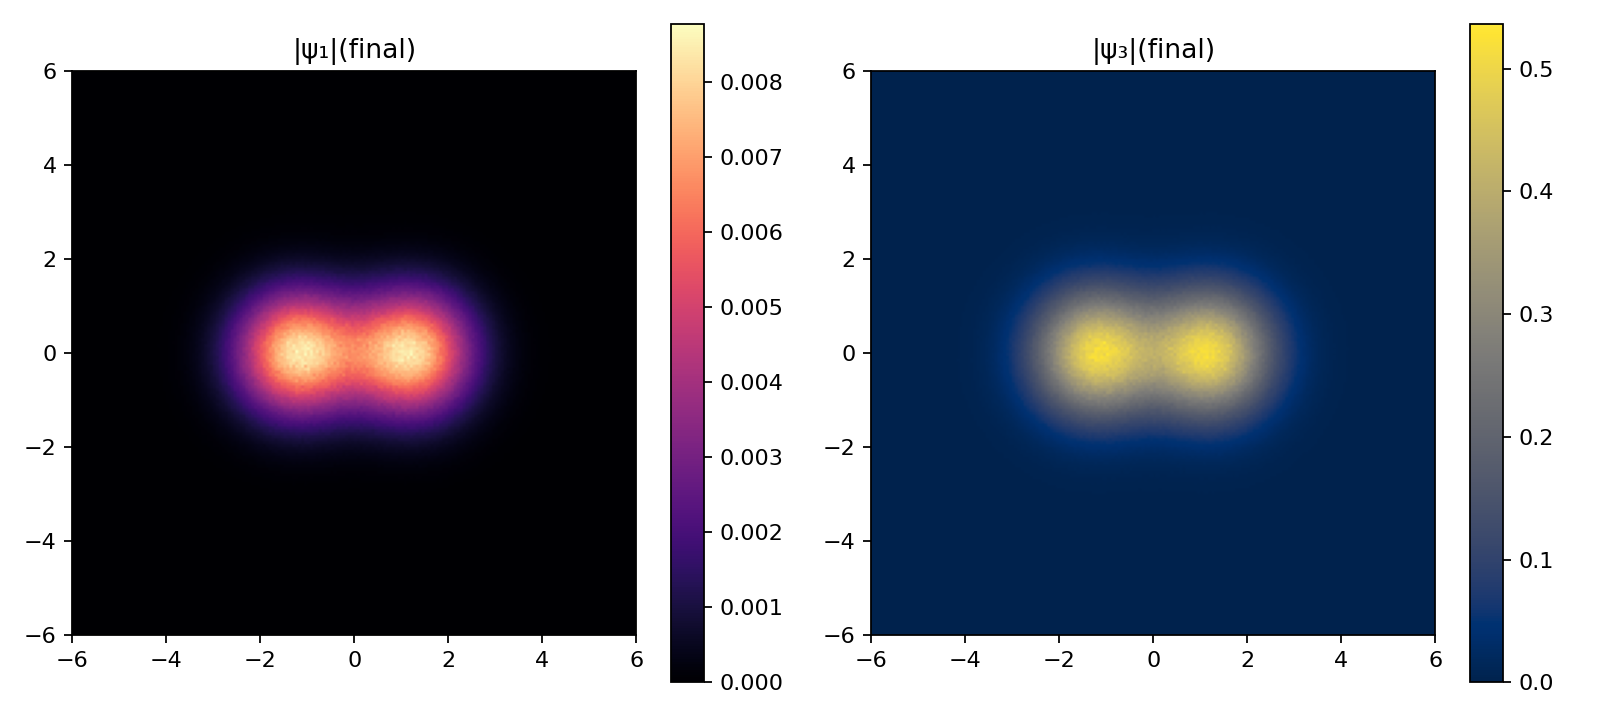
\includegraphics[width=0.48\textwidth]{PAEV_D1_VisibleHiddenMaps.png}
  \caption{Final field amplitudes \(|\psi_1|\) and \(|\psi_3|\), showing hidden curvature structure.}
\end{figure}

\end{document}